% -*- Mode:TeX -*-

%% IMPORTANT: The official thesis specifications are available at:
%%            http://libraries.mit.edu/archives/thesis-specs/
%%
%%            Please verify your thesis' formatting and copyright
%%            assignment before submission.  If you notice any
%%            discrepancies between these templates and the 
%%            MIT Libraries' specs, please let us know
%%            by e-mailing thesis@mit.edu

%% The documentclass options along with the pagestyle can be used to generate
%% a technical report, a draft copy, or a regular thesis.  You may need to
%% re-specify the pagestyle after you \include  cover.tex.  For more
%% information, see the first few lines of mitthesis.cls. 

%\documentclass[12pt,vi,twoside]{mitthesis}
%%
%%  If you want your thesis copyright to you instead of MIT, use the
%%  ``vi'' option, as above.
%%
%\documentclass[12pt,twoside,leftblank]{mitthesis}
%%
%% If you want blank pages before new chapters to be labelled ``This
%% Page Intentionally Left Blank'', use the ``leftblank'' option, as
%% above. 

\documentclass[12pt,twoside]{mitthesis}
\usepackage{lgrind}
%% These have been added at the request of the MIT Libraries, because
%% some PDF conversions mess up the ligatures.  -LB, 1/22/2014
\usepackage{cmap}
\usepackage[T1]{fontenc}
\pagestyle{plain}

%% This bit allows you to either specify only the files which you wish to
%% process, or `all' to process all files which you \include.
%% Krishna Sethuraman (1990).

%%\typein [\files]{Enter file names to process, (chap1,chap2 ...), or `all' to
%%process all files:}

%% [\files]{all}
%% \def\all{all}
%% \def\files{all}
%% \ifx\files\all \typeout{Including all files.} \else \typeout{Including only \files.} \includeonly{\files} \fi

\usepackage{hyperref}
\usepackage{graphicx}
\usepackage{tabularx}
\usepackage{listings}
\usepackage{caption}
\graphicspath{{images/}}

\begin{document}

% -*-latex-*-
% 
% For questions, comments, concerns or complaints:
% thesis@mit.edu
% 
%
% $Log: cover.tex,v $
% Revision 1.8  2008/05/13 15:02:15  jdreed
% Degree month is June, not May.  Added note about prevdegrees.
% Arthur Smith's title updated
%
% Revision 1.7  2001/02/08 18:53:16  boojum
% changed some \newpages to \cleardoublepages
%
% Revision 1.6  1999/10/21 14:49:31  boojum
% changed comment referring to documentstyle
%
% Revision 1.5  1999/10/21 14:39:04  boojum
% *** empty log message ***
%
% Revision 1.4  1997/04/18  17:54:10  othomas
% added page numbers on abstract and cover, and made 1 abstract
% page the default rather than 2.  (anne hunter tells me this
% is the new institute standard.)
%
% Revision 1.4  1997/04/18  17:54:10  othomas
% added page numbers on abstract and cover, and made 1 abstract
% page the default rather than 2.  (anne hunter tells me this
% is the new institute standard.)
%
% Revision 1.3  93/05/17  17:06:29  starflt
% Added acknowledgements section (suggested by tompalka)
% 
% Revision 1.2  92/04/22  13:13:13  epeisach
% Fixes for 1991 course 6 requirements
% Phrase "and to grant others the right to do so" has been added to 
% permission clause
% Second copy of abstract is not counted as separate pages so numbering works
% out
% 
% Revision 1.1  92/04/22  13:08:20  epeisach

% NOTE:
% These templates make an effort to conform to the MIT Thesis specifications,
% however the specifications can change.  We recommend that you verify the
% layout of your title page with your thesis advisor and/or the MIT 
% Libraries before printing your final copy.
\title{REACT: The Riskmap Evaluation and Coordination Terminal}

\author{Abraham Quintero}
% If you wish to list your previous degrees on the cover page, use the 
% previous degrees command:
%       \prevdegrees{A.A., Harvard University (1985)}
% You can use the \\ command to list multiple previous degrees
%       \prevdegrees{B.S., University of California (1978) \\
%                    S.M., Massachusetts Institute of Technology (1981)}
\department{Department of Electrical Engineering and Computer Science}

% If the thesis is for two degrees simultaneously, list them both
% separated by \and like this:
% \degree{Doctor of Philosophy \and Master of Science}
\degree{Master of Engineering in Computer Science and Engineering}

% As of the 2007-08 academic year, valid degree months are September, 
% February, or June.  The default is June.
\degreemonth{September}
\degreeyear{2019}
\thesisdate{August 20, 2019}

%% By default, the thesis will be copyrighted to MIT.  If you need to copyright
%% the thesis to yourself, just specify the `vi' documentclass option.  If for
%% some reason you want to exactly specify the copyright notice text, you can
%% use the \copyrightnoticetext command.  
%\copyrightnoticetext{\copyright IBM, 1990.  Do not open till Xmas.}

% If there is more than one supervisor, use the \supervisor command
% once for each.
\supervisor{Miho Mazereeuw}{Associate Professor}

% This is the department committee chairman, not the thesis committee
% chairman.  You should replace this with your Department's Committee
% Chairman.
\chairman{Leslie A. Kolodziejski}{Chairman, Department Committee on Graduate Theses}

% Make the titlepage based on the above information.  If you need
% something special and can't use the standard form, you can specify
% the exact text of the titlepage yourself.  Put it in a titlepage
% environment and leave blank lines where you want vertical space.
% The spaces will be adjusted to fill the entire page.  The dotted
% lines for the signatures are made with the \signature command.
\maketitle

% The abstractpage environment sets up everything on the page except
% the text itself.  The title and other header material are put at the
% top of the page, and the supervisors are listed at the bottom.  A
% new page is begun both before and after.  Of course, an abstract may
% be more than one page itself.  If you need more control over the
% format of the page, you can use the abstract environment, which puts
% the word "Abstract" at the beginning and single spaces its text.

%% You can either \input (*not* \include) your abstract file, or you can put
%% the text of the abstract directly between the \begin{abstractpage} and
%% \end{abstractpage} commands.

% First copy: start a new page, and save the page number.
\cleardoublepage
% Uncomment the next line if you do NOT want a page number on your
% abstract and acknowledgments pages.
% \pagestyle{empty}
\setcounter{savepage}{\thepage}
\begin{abstractpage}
% $Log: abstract.tex,v $
% Revision 1.1  93/05/14  14:56:25  starflt
% Initial revision
% 
% Revision 1.1  90/05/04  10:41:01  lwvanels
% Initial revision
% 
%
%% The text of your abstract and nothing else (other than comments) goes here.
%% It will be single-spaced and the rest of the text that is supposed to go on
%% the abstract page will be generated by the abstractpage environment.  This
%% file should be \input (not \include 'd) from cover.tex.

Disaster information systems use state of the art techniques in order 
to mitigate damages from natural and man made hazards. 
Developed countries utilize networks of advanced sensors and 
ahead of time mapping in order to facilitate emergency responses; 
however, such systems are not available in developing countries, which face 
the highest risk from disasters. This work seeks to use novel machine learning 
techniques to fully utilize crowdsourced social media reports gathered 
using the Riskmap system. This work establishes the motivation for using 
citizens as sensors and analyzing this noisy data using machine learning. It also 
reviews different machine learning techniques for disaster mitigation. Finally 
a novel ensemble learning model is presented that can accurately predict large 
flood events from crowdsourced data.
\end{abstractpage}

% Additional copy: start a new page, and reset the page number.  This way,
% the second copy of the abstract is not counted as separate pages.
% Uncomment the next 6 lines if you need two copies of the abstract
% page.
% \setcounter{page}{\thesavepage}
% \begin{abstractpage}
% % $Log: abstract.tex,v $
% Revision 1.1  93/05/14  14:56:25  starflt
% Initial revision
% 
% Revision 1.1  90/05/04  10:41:01  lwvanels
% Initial revision
% 
%
%% The text of your abstract and nothing else (other than comments) goes here.
%% It will be single-spaced and the rest of the text that is supposed to go on
%% the abstract page will be generated by the abstractpage environment.  This
%% file should be \input (not \include 'd) from cover.tex.

Disaster information systems use state of the art techniques in order 
to mitigate damages from natural and man made hazards. 
Developed countries utilize networks of advanced sensors and 
ahead of time mapping in order to facilitate emergency responses; 
however, such systems are not available in developing countries, which face 
the highest risk from disasters. This work seeks to use novel machine learning 
techniques to fully utilize crowdsourced social media reports gathered 
using the Riskmap system. This work establishes the motivation for using 
citizens as sensors and analyzing this noisy data using machine learning. It also 
reviews different machine learning techniques for disaster mitigation. Finally 
a novel ensemble learning model is presented that can accurately predict large 
flood events from crowdsourced data.
% \end{abstractpage}

\cleardoublepage

\section*{Acknowledgments}

To Aditya and Miho- not one page of this thesis could have been written without your
help and your guidance. Thank you so much for your patience and your expertise.

%%%%%%%%%%%%%%%%%%%%%%%%%%%%%%%%%%%%%%%%%%%%%%%%%%%%%%%%%%%%%%%%%%%%%%
% -*-latex-*-

% Some departments (e.g. 5) require an additional signature page.  See
% signature.tex for more information and uncomment the following line if
% applicable.
% % -*- Mode:TeX -*-
%
% Some departments (e.g. Chemistry) require an additional cover page
% with signatures of the thesis committee.  Please check with your
% thesis advisor or other appropriate person to determine if such a 
% page is required for your thesis.  
%
% If you choose not to use the "titlepage" environment, a \newpage
% commands, and several \vspace{\fill} commands may be necessary to
% achieve the required spacing.  The \signature command is defined in
% the "mitthesis" class
%
% The following sample appears courtesy of Ben Kaduk <kaduk@mit.edu> and
% was used in his June 2012 doctoral thesis in Chemistry. 

%% \begin{titlepage}
%% \begin{large}
%% This doctoral thesis has been examined by a Committee of the Department
%% of Chemistry as follows:
%% 
%% \signature{Professor Jianshu Cao}{Chairman, Thesis Committee \\
%%    Professor of Chemistry}
%% 
%% \signature{Professor Troy Van Voorhis}{Thesis Supervisor \\
%%    Associate Professor of Chemistry}
%% 
%% \signature{Professor Robert W. Field}{Member, Thesis Committee \\
%%    Haslam and Dewey Professor of Chemistry}
%% \end{large}
%% \end{titlepage}
%% 

\pagestyle{plain}
  % -*- Mode:TeX -*-
%% This file simply contains the commands that actually generate the table of
%% contents and lists of figures and tables.  You can omit any or all of
%% these files by simply taking out the appropriate command.  For more
%% information on these files, see appendix C.3.3 of the LaTeX manual. 
\tableofcontents
\newpage
\listoffigures
\newpage
\listoftables


%% two pager here's the problem here's how its structured
\chapter{Introduction} Natural disasters are a constant threat to societies all
over the planet. Among natural disasters, flooding is the most common calamity
in the world~\cite{chanFloodRiskAsia2012}.  Flood related deaths account for
half of all deaths from natural disasters~\cite{ohlFloodingHumanHealth2000}.
Although flooding impacts both developed and developing countries, developing
nations face much higher mortality rates as a result of flooding since they lack
resources to adequately mitigate
hazards~\cite{quarantelliUrbanVulnerabilityDisasters2003,
ahernGlobalHealthImpacts2005}. Deltaic megacities in developing countries are
particularly at risk because of unregulated urbanization, rising population, and
climate change~\cite{chanFloodRiskAsia2012}.  Moreover, there is little data
that is available before, during, and after a disaster to help stakeholders
respond to hazards~\cite{meierDigitalHumanitariansHow2015}.
% Data scarcity makes it
% hard to pinpoint where to direct aid during disasters and where to make
% infrastructure improvements after
% disasters~\cite{ranaMultidimensionalModelVulnerability2018}.

%% TODO: this is pretty disjointed
Various stakeholders, such as humanitarian Non-governmental Organizations (NGOs),
government emergency responders and affected citizens, have different but
overlapping interests with regards to disaster management.  Government and NGOs
work together to provide relief and mitigate damages from
flooding~\cite{chanResilientFloodRisk2018}, while citizens
look for relevant information and try to reduce their
risk by avoiding heavily affected
areas~\cite{viewegMicrobloggingTwoNatural2010}. Information is at the core of
disaster management; however, data scarcity makes it hard for emergency
personnel to optimize their use of resources, while citizens have an abundance
of information about their surroundings but must be careful not to trust
incorrect or outdated information about broader
areas~\cite{quarantelliProblematicalAspectsInformation1997}.

Disaster information systems can connect affected communities with
Emergency Operations Centers (EOCs), thereby bridging the information gap
between responders and citizens. Many such disaster information systems have
been developed, but they often suffer from a lack of institutional
buy-in~\cite{aminDataNaturalDisasters2008}. The lack of engagement can be partly
attributed to the difficulty of adding data gathering responsibilities to
emergency personnel that have little time during crises. One solution to this
problem is asking citizens to submit information; however, crowdsourcing brings
its own issue: in times of crisis EOCs can suffer from information overload when
they are presented with too much
data~\cite{tierneyFacingUnexpectedDisaster2001}.

In this work we present the REACT system, which uses novel machine learning and
human computer interaction research to reduce information overload from crowd
sourced data in EOCs, thereby decreasing data analysis time during disasters.
It classifies reports as indicating heavy flooding or not through an ensemble
model. It extracts key features from each of the parts of a report (text,
picture, metadata) using domain specific techniques and then uses a small dense
neural net to classify the citizen report.

First we establish the motivation for using citizens as sensors and provide an
overview of the Riskmap System which allows for gathering of citizen reports. We
then show the need for analyzing this noisy data using machine learning. A
review of different machine learning techniques that have been used in crisis
information systems, including those that also utilize social media is
presented.  Finally we describe REACT, a novel ensemble learning model that can
accurately predict large urban flood events from noisy crowdsourced data.

%% This is an example first chapter.  You should put chapter/appendix that you
%% write into a separate file, and add a line \include{yourfilename} to
%% main.tex, where `yourfilename.tex' is the name of the chapter/appendix file.
%% You can process specific files by typing their names in at the 
%% \files=
%% prompt when you run the file main.tex through LaTeX.
\chapter{Background}

%% TODO I feel like I'm restating myself here?
Global climate change is `expected to increase the frequency and intensity of
floods'~\cite{ahernGlobalHealthImpacts2005}. Developing urban areas that are
undergoing unchecked development and rising population regularly experience
flooding~\cite{chanFloodRiskAsia2012}.  Nowhere is this more apparent than
in South and Southeast Asia, where the severity of floods has been increasing
over the past several decades~\cite{tortiFloodsSoutheastAsia2012}.

Of the world's 33 mega-cities with population over 10 million, over 60 percent
are located in developing Asian
Countries~\cite{unitednationsdepartmentofeconomicandsocialaffairsWorldCities20162016}.
These cities face a looming crisis as flood risk increases, but there are also
unique opportunities for risk mitigation. Megacities are characterized by high
population density, which leads to an increase in economic damages and loss of
life during flood events, but it also means that there are large numbers of
citizens that have disaster information they would like to share with
others~\cite{chanFloodRiskAsia2012}.

\section{History of Disaster Informatics} One of the best known and earliest
work in disaster informatics was John Snow's use of maps to find the source of
the 1857 Cholera outbreak in London\cite{rogersJohnSnowData2013}. This example
is taught to all students of epidemiology and illustrates the need
not only for up to date information, but for systems that ease the
analysis of this information. In John Snow's case, the map was the technology
that allowed him to visualize the spread of the disease and effectively take
action that ended the outbreak; however, the computer revolution has drastically
changed the way that scientists and responders analyze disaster information.
John Snow used mapping technology to track the spread of disease, but now
researchers are using artificial intelligence to predict cholera outbreaks
before they happen~\cite{radinskyMiningWebPredict2013}.

%% this needs to get moved somewhere else, but I'm not sure where...
In more recent times, the need for Information Technology (IT) in disaster
management has been clear since the mid 1980s when computers became user
friendly enough to be used during
disasters~\cite{universityTerminalDisastersComputer1986}.

Now many Emergency Operations Centers (EOCs) use Geographic Information Systems
(GIS), inventory control systems, and online messaging systems among other
technology in order to organize spatial data and analyze disaster information.
For example, Mozambique used an integrated disaster management system to provide
early warning during the 2007  Zambezi floods, while Guatemala's inventory
management helped to curb government bribes~\cite{aminDataNaturalDisasters2008}.
While some systems have helped some regions to better respond to disasters,
researchers have often stated that `there are many reasons to remain skeptical
about the idea that technology will provide a panacea for emergency management
problems'~\cite{tzemosUseGISFederal1995, tierneyFacingUnexpectedDisaster2001,
perryNaturalDisasterManagement2007}. A number of potential negative effects
associated with disaster management technology have been identified: the
primarily the potential of information overload and the dissemination of
incorrect and outdated
information~\cite{quarantelliProblematicalAspectsInformation1997,
flentgeDesigningContextAwareHCI}.

\subsection{Social Media and Disasters}
%% TODO is this in the right place??
The history of online communities is firmly linked to disasters. Internet
Relay Chat (IRC) was one of the first truly global online communication systems;
its adoption among internet connected citizens was `prompted by the First Gulf
War'~\cite{salazarHashtagsAnnotatedHistory2017}. Although radio and
television broadcasts were halted by the Iraqi army shortly after the invasion,
IRC communication continued for days afterward. IRC allowed users to communicate
about conditions on the ground, including the gulf war oil spill that grew to be
the largest oil spill in history~\cite{Timeline20Years2010}.

The history of social media and the hashtag is invariably linked to disaster
communication.  It was during the San Diego bush fires of 2007 that the hashtag
was first widely used on twitter~\cite{salazarHashtagsAnnotatedHistory2017}.

Quarantelli emphasized that  `management of hazards is fundamentally social in
nature and not something that can be achieved strictly through technological
upgrading'~\cite{tierneyFacingUnexpectedDisaster2001} yet social media brings
human behavior into a machine readable format that can be used to provide
further information during disasters.

Much work has been done in passively listening to social media streams in order
to better understand how disasters unfold and how humans use social media as a
communication tool during disaster events. Many of these studies use hand
labeled tweets in order to classify what kind of information people talk
about~\cite{alamTwitterTaleThree2018}.

Further work has evolved to using artificial intelligence methods to
automatically label new tweets using supervised learning. For example, Patrick
Meier's Haiti Crisis Map initially used volunteers to classify large number of
tweets, but his more recent projects focus on the use of AI for tackling big
data problems~\cite{meierDigitalHumanitariansHow2015}.
\subsection{Crowdsourcing vs. Passive Listening} 
As Patrick Meier points out in \textit{Digital Humanitarians}, `since
humanitarian organizations don't ask eyewitnesses on social media to report
information', they must passively wait and `rely on witnesses sharing relevant
information by chance'~\cite{meierDigitalHumanitariansHow2015}. Listening to
twitter data streams and hoping that someone posts relevant disaster information
is not always a winning strategy. One solution to this problem is to have paid
workers that collect information and enter it into disaster information systems
as in~\cite{aminDataNaturalDisasters2008}, which details how paid workers were
used to input data from citizens during the Mozambique floods of 2007; however,
this method is expensive and does not scale well. The same report states that
`data processing and consolidation [were] difficult' and that `the few data
entry clerks struggled to keep up'~\cite{aminDataNaturalDisasters2008}.

%% TODO not sure where to place this section?
\section{The Riskmap System}\label{chap1:riskmap}

	\subsection{Need for open data} Creating bespoke information systems at
	the beginning of disasters has been the
	norm~\cite{aminDataNaturalDisasters2008}; however this means that
	disaster response organizations must become acclimated with the system
	at the same time that they are dealing with disaster situations.
	Researchers have shown the need to create open sourced crowdsourced
	emergency systems that provide open
	data~\cite{avvenutiNeedOpeningCrowdsourced2018a}. The Riskmap system was
	created to fill that need.


	\begin{figure} 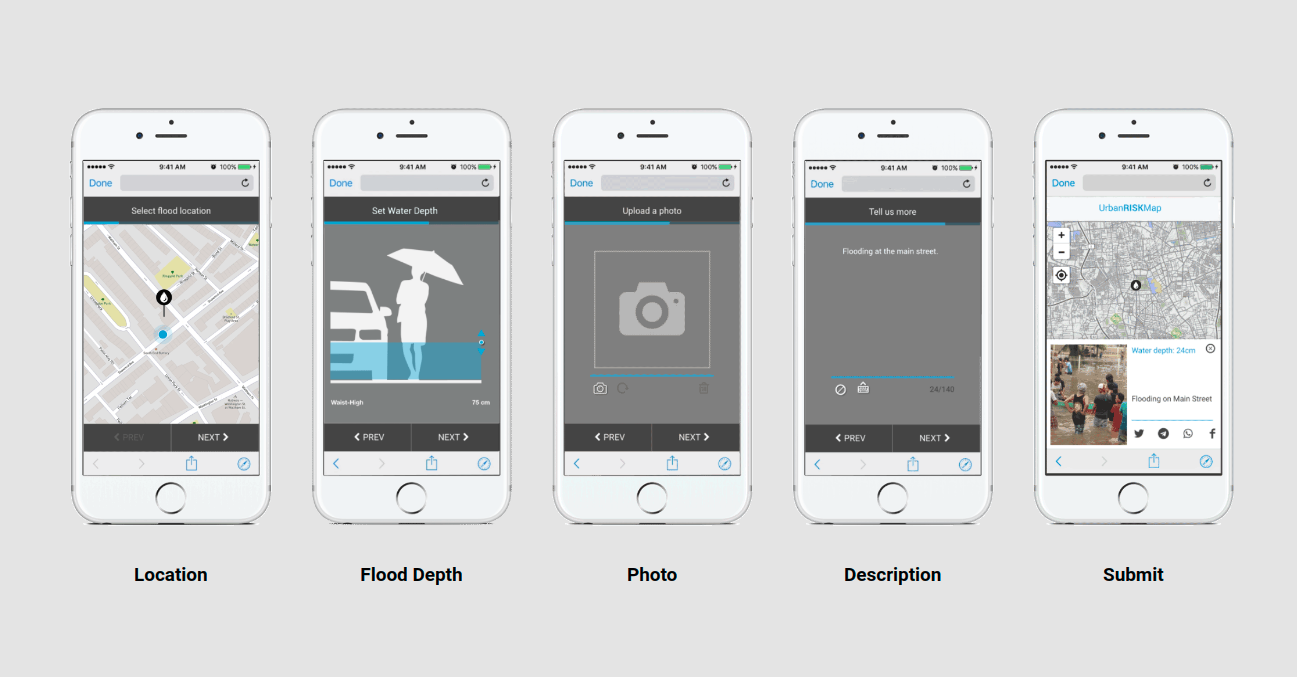
\includegraphics[width=\linewidth]{riskmap.png}
	\caption{Submitting a flood report card}\label{fig:cards} \end{figure}
	\subsection{System Overview} The Riskmap system alleviates the load on
	emergency managers by centralizing reports from many social media
	sources. It also makes it easy not only for reports to come into the
	response center, but also for emergency managers to indicate which areas
	of a city are most affected at any one time. The data gathered during an
	event is persistent and available under the Creative Commons license,
	which allows researchers to track the flood over time and pinpoint areas
	that are particularly vulnerable to flooding, thus fulfilling the need
	for open data~\cite{holdernessSocialMediaGeoSocial2015a}.

	Riskmap consists of many different social media bots that are actively
	filtering social media streams and looking for citizens that might be
	reporting flooding events, it then reaches out to those users and asks
	them to submit a flood report that consists of a GPS location, the
	estimated flood height at that location, a picture, and a textual
	description. The user interface for submitting these reports is shown
	in~\ref{fig:cards}. These reports are then displayed on a public map for other
	citizens to inform themselves. Furthermore, EOC personnel are able to
	access the Risk Evaluation Matrix (REM), a special dashboard that allows
	them to give even more information to citizens.

	The system has been in place in Jakarta and Chennai since 2016, and has
	seen hundreds of thousands of views during flood
	events~\cite{noveckOpinionElectionsWon2018, oct31ChennaiGetsRain}.

\section{Conquering Information Overload} It is not enough to create an advanced
system for consuming citizen reports, it is also necessary to ensure that this
system does not consume resources that are already scarce during a disaster
event, for example the time of emergency
workers~\cite{aminDataNaturalDisasters2008}. Furthermore, it is also important
to reduce the
resources needed to create insights because if analyzing data is too 
difficult, then decision makers will make decisions without having fully
analyzed the data~\cite{quarantelliUrbanVulnerabilityDisasters2003}.

Using computers to automatically make sense of disaster data has long
been a goal in disaster informatics, but only recently have machine
learning techniques become advanced enough to be implemented in production
emergency systems~\cite{meierDigitalHumanitariansHow2015}. Image
recognition algorithms can provide summaries of objects and scenes found
in user submitted photos~\cite{nguyenRapidClassificationCrisisRelated,
donahueDeCAFDeepConvolutional2013}. Natural language processing can
estimate the probability that a textual document is overall negative or
positive and thereby give EOCs a shorthand way to summarize thousands of
reports in short amounts of
time~\cite{nguyenRapidClassificationCrisisRelated,
nagyCrowdSentimentDetection2012}. Finally, ensemble learning methods can
learn relationships between disparate datasets and synthesize a single
result~\cite{mouzannarDamageIdentificationSocial2018}.

In this work we will experiment with different machine learning techniques
for image recognition, finally showing that transfer learning at the 
output layer can turn off the shelf multi---label  classification
algorithms into classifiers for flood image classification. For textual analysis, 
we will show the performance of bag of words, bigrams, and a combination of 
both techniques to classify report texts into heavy flooding/ no heavy flooding classes.
Flood height will first be assessed as a raw numerical feature but will then be 
joined with nearby reports through a one dimensional convolutional filter in order
to draw out temporal patterns. 

Finally, the output of these disparate techniques will be combined by using a 
small deep neural network. In order to allow better interpretability, the
most important labels from feature extraction machine learning algorithms are
presented to the user so that they can understand what drove the machine's
choice.
\chapter{Previous Work}

\section{Machine Learning in Crisis Informatics}

\subsection{Passive Listening}

Some was looking for clues after disasters:
\cite{viewegMicrobloggingTwoNatural2010}
problem: don't have real time results

Some used humans to filter out social media for real time disaster info
\cite{starbirdVoluntweetersSelforganizingDigital}
\cite{meierDigitalHumanitariansHow2015}

Some involved using machine learning:
\cite{imranPracticalExtractionDisasterrelevant2013}
\subsubsection{Problems with that approach:}
It is very difficult to filter out which social media images are related to the
disaster and which are not.


\subsection{On Image Data}
Online learning using traditional transfer
learning~\cite{donahueDeCAFDeepConvolutional2013} but online (so they get people
to label images as a disaster happens?) plus train with generic disaster
images in order to solve cold start problem at the beginning of an event.
Classify social media images into 3 classes: (severe, mild, little) damage.
\cite{nguyenDamageAssessmentSocial2017}



\subsection{On Text Data}\label{chap3:text}
Crowd sentiment detection during disasters using twitter and the 2010 San Bruno
CA fires n=3698
\cite{nagyCrowdSentimentDetection2012}

Feature engineering on twitter messages to classify into pre-incident, during
incident and post-incident
\cite{chowdhuryTweet4actUsingIncidentspecific2013}

Classifying tweets as informative/ not informative using CNNs vs SVMs (CNN wins)
\cite{carageaIdentifyingInformativeMessages2016}

CrisisNLP from the Qatar Computing Research Institute
has a huge datasets
\cite{nguyenRapidClassificationCrisisRelated}


\subsection{Ensemble Data Models}
Boosting of Tree-Based Classifiers for Predictive Risk Modeling in GIS
\cite{furlanelloBoostingTreeBasedClassifiers2000}

This paper~\cite{mouzannarDamageIdentificationSocial2018} uses deep learning to
identify damage related info 

Low level visual features (extract color, shape texture) + then Use bag of words
on the text. Make a 
\cite{jomaaSemanticVisualCues2016}

There have been some notable projects that attempt to provide complete systems
that can be used for different disasters. Most notably are the Sahana and the
AIDR projects.

Sahana has suspended its disaster response project that helped to
mobilize volunteers to respond to disasters.
// not focusing enough on the HCI and hidden wiring?


\subsection{Common Difficulties}
\subsubsection{Task Subjectivity}
Task subjectivity is an incredibly common
issue~\cite{nguyenDamageAssessmentSocial2017,
quarantelliUrbanVulnerabilityDisasters2003}. While most humans can agree on
whether an object is or is not an apple, this task does not translate to
defining if a picture indicates a severe event or a minor one. 

In other words, people's perception of risk varies widely from region to region
and from citizen to citizen~\cite{quarantelliUrbanVulnerabilityDisasters2003}.

\subsubsection{Small Datasets}
Although larger datasets have recently become available, there has
historically been a scarcity of training and validation data available for
Deep learning models that are trained on small datasets tend to overfit on the
training data and do not generalize well to the validation
dataset~\cite{perezEffectivenessDataAugmentation2017}.

In many early studies only hundreds of data points were considered--- combined
with the small size of those data points (for example, twitter microblogs of
140 or 280 characters) and effectively using deep learning becomes very
difficult.
% TODO for Adi should I not write this? % 
For example~\cite{nagyCrowdSentimentDetection2012} only uses 3,698 tweets in
order to train 

\subsubsection{Connects citizens to EOC}
As discussed in~\ref{chap1:riskmap}, the Riskmap system helps to connect
citizens to Emergency Operations Centers

\subsubsection{Focus on technology rather than whole system design}
A series of UN case studies on six disaster information systems found that while
engineering and system design were essential, it was the hidden wiring of support
networks that allows for technology to succeed.

\begin{quote}
An important message emerges from the case studies: an effective disaster
information management system requires a good technological platform,
but also much more. Software programs for storing, sharing, and manipulating
data for disasters are being developed or patched together at a steady pace,
often in the aftermath of disasters. The real difficulty lies in anchoring
these technological approaches in an appropriate institutional context where
they are supported by relevant and effective operating procedures, agreed
terminology and data labeling, and a shared awareness of the benefits of proper
handling of disaster information. Clearly, a disaster information management
system must be supported by accepted rules, procedures, and relationships
that encourage, facilitate, and guide the production, sharing, and analysis and
use of data in response to disaster. In these case studies, the institutional
dimension---the hidden wiring---determined the effectiveness of the
systems.~\cite{aminDataNaturalDisasters2008}
\end{quote}


\chapter{Methodology and Results}
The Riskmap system allows citizens to easily submit
disaster reports as such it has allowed the Urban Risk Lab at
MIT to gather thousands of reports of real flooding in Indonesia and India.
These data points include requests for help, traffic reports, indications that an
area is safe, and advice for other citizens in the area. Images attached to
reports include a wide variety of scenes, from daylight highways with cars and
motorcycles to night time deserted alleys. Additionally, citizens were asked to
provide an estimated flood height using a slider.

\section{Text}
As shown in Section~\ref{chap1:riskmap}, the Riskmap system allows citizens to provide
a textual description to emergency managers. In Indonesia, most of the reports
are provided in Bahasa, the local language; however, in Chennai all reports were
submitted in English even though the system also supports Tamil. In both Chennai
and Jakarta these reports are quite brief, with the longest reports having 140
characters. In this manner, they are quite similar to tweets which were
initially 140 characters but this limit was doubled in 2017. Helpfully, this
means that much of the work described in~\ref{chap3:text} applies to the Riskmap
text corpus.

Table~\ref{table:text_sample} contains a sample of ten reports that are
indicative of those found in the Riskmap textual descriptions.

\label{table:text_sample}
\begin{table}
  \begin{tabular}{ll}
    \toprule
    {} &
    text \\
    pkey &
    \\
    \hline{}
    \midrule
    169  &
    Waterlogging near cathedral road flyover  \\
    171  &
    1st street Engineers avenue \\
    173  &
    Not that much water safe only \\
    174  &
    50cm water stagnant on the road \\
    176  &
    Water level rising  slowly  \\
    177  &
    Water logging  \\
    178  &
    Model school road is completely flooded, with water almost knee deep \\
    179  &
    Heavy rain in West mambalam flood \\
    180  &
    Water on roads. Stay safe \\
    182  &                                                           4cm
    rainfall.. still continuing.. hope for safe .. dont come outside in
    night time \\
    181  &
    Luz signal flooded knee deep water \\
    \bottomrule
  \end{tabular}
\end{table}

\subsection{Preprocessing}
We first remove test reports, which are reports submitted in order to ensure
that the system is working. The following POSTGRESQL query was executed to remove
reports that were only used to test the system:

\begin{lstlisting}[language=SQL]
SELECT   pkey,
         text
FROM     riskmap.all_reports
WHERE    text IS NOT NULL
AND      Length (text) > 0
AND      text NOT similar TO '%%(T|t)(E|e)(S|s)(T|t)%%'
ORDER BY created_at;
\end{lstlisting}

We then use python to remove punctuation and then split along whitespace, thus
splitting the source text into individual words without any spaces.

\begin{lstlisting}[language=python]
def prepare_text(report_text):
    '''
    returns a list of strings where each string is a different word
    '''
    import string
    exclude = set(string.punctuation)
    s = "".join(ch for ch in inp if ch not in exclude )
    return s.lower().split()
\end{lstlisting}

\subsection{Sentiment analysis}
Since each report in the Chennai dataset includes a textual description in English,
we could use off the shelf sentiment analysis to gauge how
negatively citizens are feeling. It might be the case that a highly negative
sentiment corresponds to heavy flooding and that a positive sentiment
corresponds to lighter or no flooding.  We can investigate the relation between
a negative sentiment and heavy flooding by using conditional probability. We set
the threshhold for negative sentiment at~.5 and then use the AWS Rekognition API
in order to classify texts into heavy flooding when negative sentiment is
greater than $.5$ and into light or no flooding otherwise.

We use bayes' rule in order to analyze the true positive rate--- the
probability that a report represents heavy flooding given a negative sentiment:
\\
$$P( Heavy Flooding | negative) =  \frac{P(heavy Flooding | negative)}{P(negative)} =.65 $$
\\

The false positive rate, which is the probability that there is no heavy
flooding given a negative sentiment is given by:

\\
$$P( No Flooding | negative) =  \frac{P(No Flooding | negative)}{P(negative)} =.34 $$
\\

These probabilities show that while there is some relation between a negative
sentiment and flooding, it is not a very strong signal. Furthermore, there are
no off the shelf sentiment analysis tools for the Indonesian language, so a
model based on AWS Rekogniton or Google Cloud Natural Language API would not
translate to the Jakarta dataset.

\subsection{Bag Of Words}
While sentiment analysis might not be a strong enough signal of heavy flooding/
no heavy flooding, our experiment shows that the textual data contains important
information. In order to train a machine learning algorithm on textual data one
must first create an embedding that maps natural language into feature vectors.
There are many ways of creating embeddings as discussed in
Section~\ref{chap3:text}, but many of them require large datasets or do not
support Indonesian. For example, word2vec is a popular embedding model that
produces floating point vectors and has achieved remarkable performance;
however, the size of its training vocabulary is 962,000 unique
words~\cite{mikolovDistributedRepresentationsWords2013}. It is possible to
download a pre-trained word2vec model and use it to encode new texts, but such a
pre-trained model doesn't exist for Indonesian. We could train it using a
different dataset of Indonesian texts, but there is no guarantee that our domain
specific words would have a good embedding after having trained with a different
corpus.

The bag of words encoding is particularly attractive to the Riskmap
dataset because it language agnostic and can therefore work on both the Chennai
and Jakarta datasets.  The bag of words approach to classifying texts consists
of first creating a vocabulary that maps from a token t to a unique index i. Each
report text is then encoded into a feature vector by setting the ith element to
1 if the token t exists in the report
text~\cite{khuranaNaturalLanguageProcessing2017}.

The bag of words model correctly classifies 67 percent of reports in the Chennai corpus
under 5 fold cross validation. Examining the data, we see that there are many
instances of reports such as `no flooding here' which are being
misclassified because the embedding is not able to understand relationships
between adjacent words.

\subsection{Bigrams}
Bigrams are an embedding that allows the separator to learn relationships
between adjacent words. The vocabulary is created by using pairs of adjacent
words, such that `no flooding here' would turn into 2 tokens: `no flooding' and
`flooding here'.

\subsection{Both}


\section{Images}

\subsection{Visual Bag of Words}

~\cite{yangEvaluatingBagofvisualwordsRepresentations2007}

\section{Flood Height}
\subsection{Raw}
\subsection{Normalized}

\section{Ensemble with Neural Net}
In~\cite{jordanHierarchicalMixturesExperts1994}, Jordan and Jacobs showed that
nueral networks can be effectively used to vote between different classifiers
that are effictive only in their specific domain of the space. They present a
case for using the Estimation Maximization (EM) algorithm for optimizing the
weights of the neural network.
Hierarchical mixtures of experts and the EM
algorithm~\cite{jordanHierarchicalMixturesExperts1994}
+ bishop p. 673~\cite{bishopPatternRecognitionMachine2006}

\chapter{Future Work}

\section{Image Data}
\subsection{Using transfer learning}
As the time goes on and the Riskmap System registers more flood events, 
more data will be collected, thereby increasing the  

\section{Text Data}
\subsubsection{word2vec}
As outlined previously, we did not experiment with word2vec embeddings because
of the difficulty of handling multilanguage datasets; however, it would be
possible to create a word2vec embedder for Indonesian by using publicly
available texts such as Wikipedia. The short coming of using Indonesian Wikipedia 
is that there are only 500 thousand articles compared to 5.9 million in English Wikipedia.

\section{Flood Height}
\section{Location Information}

\section{Ensemble Methods}
\subsection{Bigger network}
Our current bagging network is very small so as to reduce over fitting on the
small datasets we currently have. As the Riskmap System collects more data, it
is likely that we can use a larger network with a decreased risk of over fitting.

\subsection{Data Augmentation}
It might be possible to use generative adversarial learning in order to create
new example reports that fit into the distribution of user submitted reports.
This would increase the size of the dataset without having to deploy the
Riskmap system to more locations. One of the challenges related to
generating new reports would be the multi-language problem and validating
that generated report texts in other languages fit the distribution of user
submitted reports in that language.

% TODO conclusion
\chapter{Conclusion}

\appendix
\chapter{Tables}

Place tables here.

\newpage

\chapter{Figures}

\vspace*{-3in}

Place figures here
\newpage

%% This defines the bibliography file (main.bib) and the bibliography style.
%% If you want to create a bibliography file by hand, change the contents of
%% this file to a `thebibliography' environment.  For more information 
%% see section 4.3 of the LaTeX manual.
\begin{singlespace}
\bibliography{main}
\bibliographystyle{plain}
\end{singlespace}

\end{document}

